\documentclass[12pt]{ib102}
\usepackage[czech]{babel}
\usepackage{graphicx}

\setassignment{2}
\setexercise{1}
\setduedate{30}{9}{2013}
\setpoints{2}

%%% ZDE NAPISTE SVOJE UCO, JMENO A SKUPINU
\setstudent{Jan Tušil}
\setgroup{MI6}
\setuco{410062}


\begin{document}

\begin{zadani}
Mějme následující jazyk:
\begin{align*}
L = \{w \in \{l,o,s\}^* \mid &\text{ každý výskyt podslova } los \text{ ve slově } w \\
&\text{ se nachází uvnitř podlova } losos \}
\end{align*}
Sestrojte totální deterministický konečný automat přijímající jazyk $L$.
\end{zadani}

\begin{reseni}
\begin{figure}[h!]
\centering
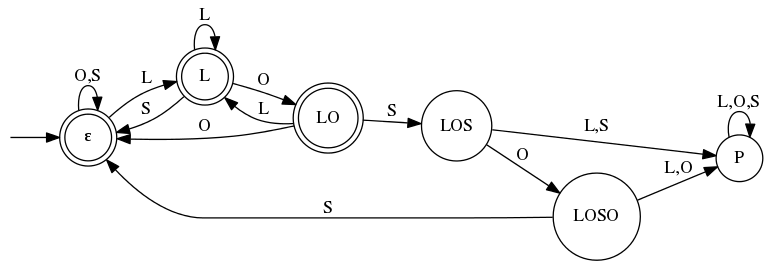
\includegraphics[width=0.8\linewidth]{losos.png}
\caption{DFA, přijímající jazyk \( L \)}
\end{figure}
\end{reseni}

\end{document}
